\runningheader{Oppgave d)}{}{Side \thepage\ av \numpages}
% ********************************************************
% oppgave d) 
% ********************************************************  
\item
{\bf Numerisk integrasjon som Matlab-funksjon}
\label{oppg:d}

I denne oppgaven skal du lage en egen funksjon av
Eulers forovermetode for numerisk integrasjon.
Du kan også velge å gjøre en frivillig ekstraoppgave hvor du
implementerer alle tre metodene for numerisk integrasjon, og spesifiserer i
funksjonskallet  hvilken metode du vil bruke.
For introduksjon til
funksjoner i Matlab, skriv {\color{red}\fbox{\tt doc function}} i {\tt Command Window}. 



  \begin{itemize}
  \item  Koden i skallfilen kaller på
    funksjonen {\tt EulerForover} som vist under
\begin{lstlisting}[caption={Kodeutdrag som kaller på funksjonen {\tt EulerForover}.},
language= Matlab, label=kode:funksjon_EF,
numbers=none]
y(1) = 0;  % initialverdi
for ..
    y(k) = EulerForover(.. , .., ..);
end
\end{lstlisting}

Med utgangspunkt i Eulers forovermetode gitt som
\begin{equation}
  \label{eq:1aa}
  y_{k}  =  y_{k-1} +  T_s {\cdot} u_{k-1}
\end{equation}
fullfør koden i skallfilen til funksjonen  
\fbox{\tt  EulerForover.m}, gjengitt under.

\begin{lstlisting}[caption={Funksjonen/filen {\tt EulerForover.m}.},
language= Matlab, label=kode:funksjon_EF2,
numbers=none]
function IntValueNew = EulerForover(IntValueOld, Timestep, FunctionValue)
% fyll inn
end
\end{lstlisting}

    Som du ser benytter funksjonen variabelnavn som er matematisk  
    beskrivende, samtidig som at den ikke skal benytte indeks
    {\tt k}.

    \item Kjør koden  og vis at {\tt y(k)} gir samme resultat som 
    {\tt  y\_EulerF(k)} i oppgave~\ref{oppg:b}).
\end{itemize}


    

\newpage
\subsubsection*{Generell funksjon for numerisk integrasjon (frivillig)}

For å ha en mer fleksibel integrasjonsrutine skal vi lage en ny
funksjon hvor vi inkluderer et argument som sier noe om hvilken
metode som skal brukes.
Et utgangspunkt for dette er funksjonen {\tt Integrasjon} vist i
kode~\ref{kode:funksjon_num_int}, og  
denne finner du igjen i skallfilen \fbox{\tt Integrasjon.m}.
  

\begin{lstlisting}[caption={Den utvidede funksjonen/filen {\tt Integrasjon.m}.},
language= Matlab, 
label=kode:funksjon_num_int,
 numbers=none]
function IntValueNew = Integrasjon(IntValueOld, Timestep, FunctionValues, options)

arguments
    IntValueOld (1,1) double             % spesifiserer som skalar, 1x1
    Timestep (1,1) double                % spesifiserer som skalar, 1x1
    FunctionValues (1,2) double          % spesifiserer som vektor, 1x2
    options.metode (1,:) char = 'Trapes' % metodevalg, default er Trapes
end
    
if strcmp(options.metode,'EulerForover')
    % fyll inn
elseif strcmp(options.metode,'EulerBakover')
    % fyll inn
elseif strcmp(options.metode,'Trapes')
    % fyll inn
else
    errordlg('Feil metode spesifisert')
    return
end
end
\end{lstlisting}

For å kalle på denne 
funksjonen benyttes syntaksen vist i
kode~\ref{kode:funksjon_num_int_kall} hvor du ser at de to siste elementene
{\tt  u(k-1:k)} sendes inn, uansett  metodevalg. Du må derfor passe å plukke ut riktig
element for hver metode i funksjonen.  

\begin{lstlisting}[caption={Alternativ bruk av funksjonen {\tt Integrasjon}.},
language= Matlab,  label=kode:funksjon_num_int_kall,
linewidth=13.5cm, numbers=none]
y(k) = Integrasjon(y(k-1), T_s, u(k-1:k), metode='EulerForover');
y(k) = Integrasjon(y(k-1), T_s, u(k-1:k), metode='EulerBakover');
y(k) = Integrasjon(y(k-1), T_s, u(k-1:k), metode='Trapes');
y(k) = Integrasjon(y(k-1), T_s, u(k-1:k));   % default: Trapes
\end{lstlisting}

 Vis at ved å kjøre koden så får du resultatet vist i figur~\ref{fig:3d3}. 

\begin{itemize}
  \item Lek litt med å øke og/eller redusere på steglengden \fbox{\tt
      T\_s} i linje 5, og studer effekten på integralene.   
\end{itemize}



    \begin{figure}[H]
      \centering
      \hspace*{0mm}\scalebox{0.6}{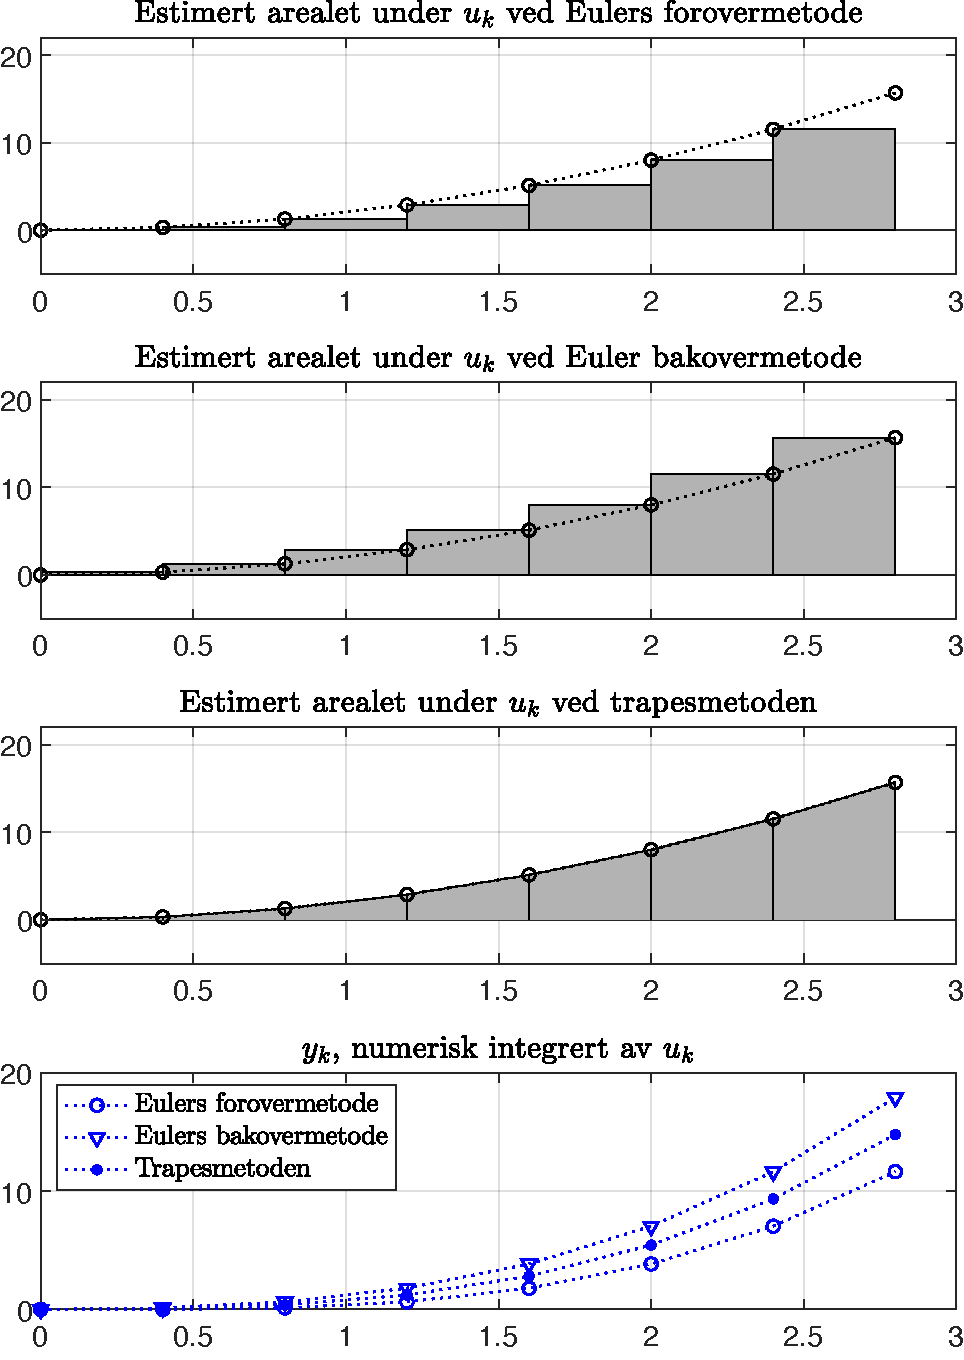
\includegraphics{fig3d_2.pdf}}
      \caption{Presentasjon av arealet under  kurven $u_{k}$ for de
        tre integrasjonsmetodene ved å bruke henholdsvis 
        {\color{red}\fbox{\tt bar}} og {\color{red}\fbox{\tt area}}-kommandoene.}
      \label{fig:3d3}
    \end{figure}

